\documentclass{article}
\usepackage{fancyvrb}
\usepackage{xspace}
\usepackage{framed}
\usepackage{theorem} % theorembodyfont
\usepackage{amsmath} % \cfrac
\usepackage{amssymb} % \mathbb
\usepackage{graphicx}
\graphicspath{ {pic/} }

\begin{document}
\title{KaSa note}
\maketitle

% environments
\renewenvironment{i}{\begin{itemize}}{\end{itemize}}
\newenvironment{e}{\begin{enumerate}}{\end{enumerate}}

% arrows
\renewcommand\a{\rightarrow}
\newcommand\A{\Rightarrow}
\renewcommand\aa{\leftrightarrow}
\renewcommand\AA{\Leftrightarrow}
\newcommand\la{\leftarrow}
\newcommand\lA{\Leftarrow}
\newcommand\ad{\downarrow}
\newcommand\Ad{\Downarrow}
\newcommand\au{\uparrow}
\newcommand\Au{\Uparrow}
\renewcommand\to{\mapsto}

\newcommand\tool[1]{\textsf{#1}\xspace}

% picture
\newcommand\g[2][]{\includegraphics[#1]{pic/#2}}

\newcommand\kasa{\tool{KaSa}}
\newcommand\kapa{\tool{Kappa}}

%%%%%%%%%%%%%%%%%%%%%%%%%%%%%%%%%%%%%%%%%%%%%%%%%%%%%%%%%%%%%%%%%%%%%%%
\section{Goal}

The goal is to offer a programming/modelling environment for the language
\kapa, a grap rewrite language that can be used to describe models of
biological systems such as signalling pathways.

The first year will focus on the design of a causal compression tool (that
computes minimal sub-traces) and a static analyser that computes invariants
about the bio-molecular species (or a graph components) that can arise in
model and provide debugging information.

%%%%%%%%%%%%%%%%%%%%%%%%%%%%%%%%%%%%%%%%%%%%%%%%%%%%%%%%%%%%%%%%%%%%%%%
\section{KaSa}

\kasa is a high level rule-based language designed to describe
Protein-Protein networks.  Rule-based language where physical reactions
convert to rules.  In \kapa, there is no change in the configuration of the
system without the execution of a rule. There are five fundamental points
to a \kapa language:

\begin{e}
\item Agents: represent the consistent molecules of a system. Agents are
  population number and the characterised having binding sites.
\item Tokens: concentration and do not have binding sites.
\item Rules: bio-chemical process (have agents/tokens or both).
\item Rates: determines the number of times the rule is applied for each
  instance of the rule. Each rule has an initial condition which must be
  satisfied for the rule to be valid. If the conditions are met, the rule
  is applied according to the rate.
\item Observables: determines the output data in terms of either agent
  count or token concentration.
\end{e}

The syntax of \kapa:

\begin{framed}
\begin{i}
\item Rule in English: "unphosphorylated site 1 of agent A binds to site 1 of
agent B".
\item \kapa rule: \verb|A(site1~u), B(site1) -> A(site1~u!1), B(site1!1)|
\end{i}
\end{framed}

\begin{i}
\item Agents: name, number of interaction sites, internal state
  \verb|A(x~u,y), B(x), ...|
\item Sites: multiple sites are separated by a comma, \verb|A(s1,s2,..)|
\item States: binding state and internal state (\verb|~u, ~p|). \verb|~u|:
  an unphosphorylated state; \verb|~p|: an phosphorylated state.
\item Bonds:
\begin{i}
\item \verb|!|: specified the physical bonds using shared indicate across
  agents to indicate the 2 end points of a link.
\item \verb|!_|: does not care bond to whom. Only said that this site is
  bound. It is called an any bound.
\item \verb|?|: withcard bound. This used when when one is tracking
  modification sites.
\end{i}
\end{i}

\begin{figure}[ht!]
\centering
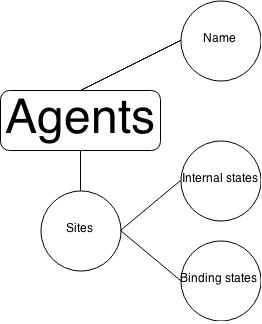
\includegraphics[width=40mm]{agents.jpg}
\caption{An agent component \label{agent}}
\end{figure}

For example: \verb|A(x, y~u~p, z~0~1~2)|\\

The agent \verb|A| with 3 interaction sites (\verb|x, y, z|); which site
\verb|y| possessing 2 internal states (\verb|~u, ~p|); the site \verb|z|
having 3 possible states (\verb|0,1,2|). State can be character or integer.

\kapa models how structures called "mixture" are affected by rules. A
mixture describes the state of "sites" on entities called "agents".

Rules are applied to transform mixtures. Each rule consists of 3 "site
graphs" (pattern): a left-hand side, a domain of definition, a right-hand
side. A rule can be applied when its left-hand side is matched in the
mixture. The domain of definition is a sub-pattern of the left-hand
side. Anything matched by something in the left-hand side outside the
domain of definition is deleted by application of the rule.

A \kapa model consists of a collection of concrete agents and rules. Each
agent, or more properly agent type has a "name", an associated set of
"sites", each with optional internal state and a "copy number". An atomic
rule falls into one of 5 classes:

\begin{i}
\item a binding between 2 agents.
\item an unbinding.
\item the modification of an agent.
\item the creation of an agent.
\item the deletion of an agent.
\end{i}

\begin{figure}[ht!]
\centering
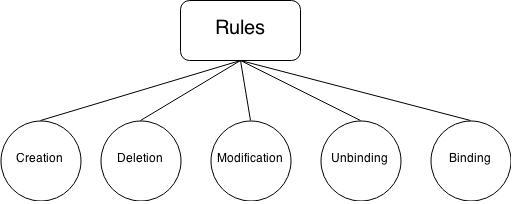
\includegraphics[width=80mm]{rules.jpg}
\caption{A rule component \label{rule}}
\end{figure}

But a rule can be non-atomic, it can combining several actions.

Given a \kapa model, its "contact map", which is computed statically from
the rules, specifies which agents can bind and on which sites.

Its "influence map" also computed statically, specifies the causal
relations of activation and inhibition between rules, that is to say a rule
activates (inhibits) another if its application may addd (subtract) from
the set of instances of the other one.

%%%%%%%%%%%%%%%%%%%%%%%%%%%%%%%%%%%%%%%%%%%%%%%%%%%%%%%%%%%%%%%%%%%%%%%
\section{Kappa syntax}

TODO\\

Rules in \kapa syntax:

- Add, remove, delete, bind (only two agents): agents, sites, etc.



%%%%%%%%%%%%%%%%%%%%%%%%%%%%%%%%%%%%%%%%%%%%%%%%%%%%%%%%%%%%%%%%%%%%%%%
\section{KaSa test}

The current implementation of the influence map has the following
limitations:
\begin{i}
\item Only observables that are defined as patterns are taken into account.
\item Not atomic observables which are defined as algebraric expressions
  are not taken into account yet. The observables are ignored.
\item The influence map does not take into account indirect influences due
  to perturbations (which could arises when the application of a rule
  triggers a pertubation which would create some agents or
  increase/decrease the value of some variables).
\item Token are not taken into account yet. They are currently ignore.
\item Positive/negative influence of time is not taken into account either.
\end{i}


%=======================================================================
\subsection{Signatures}

\begin{i}
\item Agents
\item Sites: binding state, internal state (\verb|~u, ~p|)
\item States: it can be
\begin{i}
\item Free
\item Connect to another agents at some sites
\item Internal states
\end{i}
\item Duals
\end{i}

For example: \verb|abc.ka|

\begin{i}
\item Agents:

\begin{verbatim}
Signature:agents:
Signature:agents:0:A
Signature:agents:1:B
Signature:agents:2:C
\end{verbatim}

  where \verb|agent_index:agent_name| is an index of that agent

\item Sites:

\begin{verbatim}
C(x1~u~p, x2~u~p)

Signature:sites:2:
Signature:sites:2:0->x1 (internal state)
Signature:sites:2:1->x2 (internal state)
Signature:sites:2:2->x1 (binding state)
Signature:sites:2:3->x2 (binding state)
\end{verbatim}

  where \verb|agent_index:site_index->state_name|

\item States:

\begin{verbatim}
Signature:states:2:
Signature:states:2:0:
Signature:states:2:0:0->u
Signature:states:2:0:1->p

Signature:states:2:2:
Signature:states:2:2:0->free
Signature:states:2:2:1->0@1  // agent@site
\end{verbatim}

  where
  \verb|agent_index:site_index:state_index->states_name|. \verb|state_name|:
  it can be \verb|internal state|, \verb|free|, or connect to another agent
  \verb|agent_id@site_id|.

  \verb|Signature:states:2:2:1->0@1|: agent 2 at site 2 has state 1 is a
  connection of agent 0 at site 1.

\item Duals:

\begin{verbatim}
Signature:duals:0:
Signature:duals:0:0:
Signature:duals:0:0:1:
Signature:duals:0:0:1:1,0,1
\end{verbatim}

  where
  \verb|agent_index:site_index:state_index:agent_index,site_index,state_index|

\verb|Signature:duals:0:0:1:1,0,1|: agent 0, site 0, state 0: agent 1, site
0, state 1
\end{i}

%=======================================================================
\subsection{Compilation}

\begin{i}
\item Variables: do not print the pattern, only print the value.

\item Rules:
 \begin{i}
  \item Left-hand side
  \item Right-hand side
  \item Direct: lhs different
  \item Reverse:rhs different
  \item Bonds
  \item Actions:
   \begin{e}
     \item Binding
     \item Unbinding
     \item 1/2 unbinding
     \item Creation
     \item Deletion: documented\_site, undocumented\_site
   \end{e}

\end{i}

\item Initial states

\end{i}

For example:

\begin{i}
\item LHS: the lhs of rule 0, \verb|agent_id_0|: index of lhs rule 0,
  \verb|agent_type_1|: agent index 1, \verb|site_type_0|: site index is 0,
  \verb|state:[0;0]|: is of state \verb|[state_index_min, state_index_max]|
\begin{verbatim}
rules:0:lhs:agent_id_0:agent_type_1:site_type_0 ->state:[0;0]
\end{verbatim}

\item Binding, unbinding:

\begin{verbatim}
rules:0:actions:binding:(1,0)@0 ---- (0,1)@0 // (agent_id,agent_type)@site
\end{verbatim}

  rule 0 has an action binding: (agent\_index, agent\_id)@site. Rule 0 has
  (agent 1, position 0)@site 0 connect to (agent 0, position 1)@ site 0.

\item 1/2 unbinding:

\begin{verbatim}
rules:1:actions:1/2unbinding:(0,0)@0
\end{verbatim}

rule 1 has an action 1/2 unbinding at (agent\_id 0, agent\_type 0)@site 0.

\item Deletion:

\begin{verbatim}
rules:0:actions:deletion:(0,1) // (agent_id, agent_type)
rules:0:actions:deletion:documented_site:(0,1)@0  // (agent_id, agent_type)@site
rules:0:actions:deletion:undocumented_site:(0,1)@1
\end{verbatim}

  rule 0 has an actions deletion at agent\_id 0, agent\_type 1. Where the
  site is documented at site 0.

\item Creation:
\begin{verbatim}
rules:0:actions:creation:(0,2)
\end{verbatim}

rule 0 has an action creation at (agent\_id 0, agent\_type 2).

\end{i}

%=======================================================================
\subsection{Quarks}
Compute the influence relations between rules and sites.

\begin{figure}[ht!]
\centering
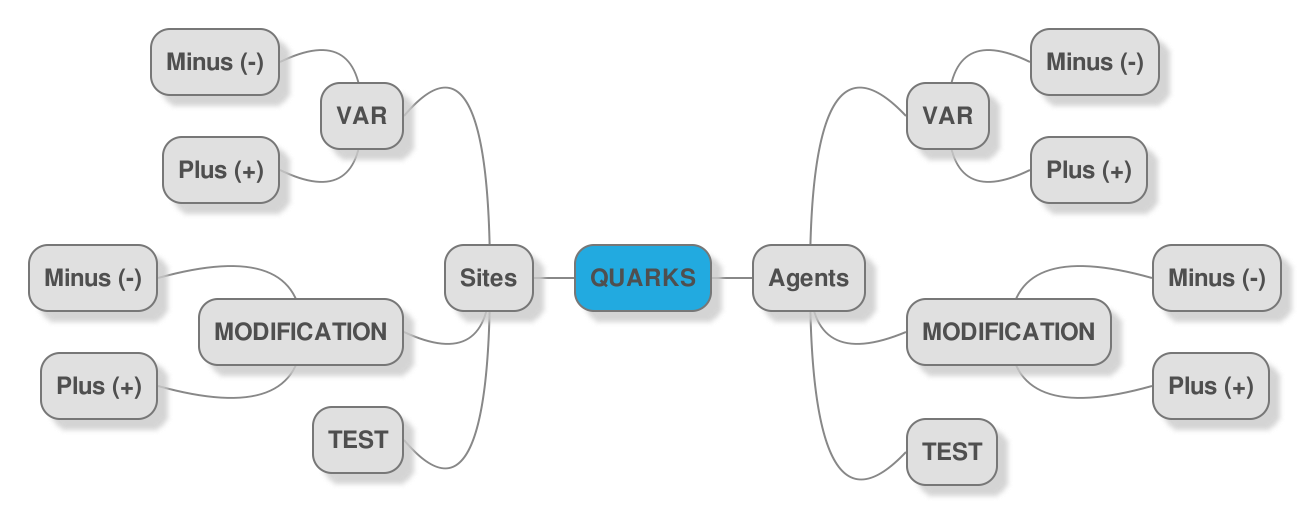
\includegraphics[width=110mm]{quarks.png}
\caption{A quark component \label{quark}}
\end{figure}

\begin{e}
\item TEST: what is tested in the left-hand side.
\item CREATION: the agents that are created.
\item REMOVAL. the agents that are removed.
\item MODIFICATION +: the sites that are directly modified (excluding
  site-effects)
\item MODIFICATION -: the sites that are directly modified (excluding
  site-effects)
\item VAR
\end{e}

For example:
\begin{i}

\item TEST
\begin{verbatim}
Quarks:Rule 0
Quarks:TEST
Quarks:00   // rule 0, agent 0
Quarks:0001 // rule 0, agent 0, site 0, state 1
\end{verbatim}

\item CREATION
\begin{verbatim}
Quarks:CREATION
Quarks:20 // rule 2, agent 0
\end{verbatim}

\item REMOVAL
\begin{verbatim}
Quarks:REMOVAL
Quarks:20 // rule 2, agent 0
Quarks:2010 // rule 2, agent 0, site 1, state 0
\end{verbatim}

\item MODIFICATION +/-: rules modified rhs/lhs

\item VAR
\begin{verbatim}
Quarks:Var 3 // variable 3
Quarks:30 // variable 3, agent 0
Quarks:3001 // variable 3, agent 0, site 0, state 1
\end{verbatim}

\end{i}

%----------------------------------------------------------------
\subsubsection{Quarks map}

\begin{i}
\item Agent
  \begin{i}
    \item var+: variable on the rhs rule
    \item var-: variable on the lhs rule
    \item test
    \item modif+: rule modified on the rhs
    \item modif-: rule modified on the lhs
  \end{i}

\item Site
  \begin{i}
    \item vars+
    \item vars-
    \item test
    \item modif+
    \item modif-
  \end{i}

\end{i}

For example: \verb|create2.ka|

\begin{verbatim}
Quarks:agent_test**:agent_type:0, rule: 1 -> [0;1] // rule 1 [position 0;
position 1]
Quarks:site_modif+**:agent_type:0,site_type:0, state:0,
  rule : 1 -> [-2;0]
\end{verbatim}

Remarks If a position is a negative number [-i], then it refers an agent
that is connected to the agent at position (i-1) that is modified by side
effects.
%----------------------------------------------------------------
\subsubsection{Context map}

The contact map summaries the different types of agent, their interface and
the potential binding between sites.

Q: How to compute the context map?\\
It is compute statically and does not depend on the kinectic rates nor
initial conditions.

%----------------------------------------------------------------
\subsubsection{Influence map}

The influence map of a model is an object that may help modellers checking
the consistency of the rule set they use.

It describles how rules may potentially influence each other during a
simulation.

The influence map will not display relations between rules that are
included by site effects.

Observables have no influence, but they can be influenced by rules, if the
rule can increase or decrease their value.

Observables are represented as circular nodes, and rules as rectangular
nodes. Edges are decorated with the list of embeddings (separated by a
semi-colon) allowing rules' right hand sides to be mapped to left-hand
sides.

For example: \verb|[1->0]|: right hand side of a first rule/var at position 1 has
influence to the left hand side of a second rule/var at position 0.

\begin{i}
\item Wake up map: positive influence (create)
\item Inhibition map: negative influence (destroy)
\end{i}

Give example of wake up map and inhibition map:

Q: How to compute the influence map?

It is statically computed and does not depend on kinetic rates nor initial
conditions.

%----------------------------------------------------------------
\subsubsection{Site effect}

%----------------------------------------------------------------
\subsubsection{Adding and deleting agents}


%=======================================================================
\subsection{Annotated map}


%----------------------------------------------------------------
\subsubsection{Qualitative analysis}

Compute the subset of sites which occurs together in the left-hand site of
a rule; among them only keep the maximal ones.


%----------------------------------------------------------------
\subsubsection{ODEs-Ordinary Differential Equations}

Annotate the contact map with the projection of the flow of information.

ODEs would be highly useful for rapidly exploring system dynamics by
numerical integration; but a flat-out expansion of rules into ODEs would,
of course, fall victim to the combinatorial explosion.

Give example of ODEs:


%----------------------------------------------------------------
\subsubsection{CTMCs-Continuous-Time-Markov-Chain}

Compute one partitioning of the sites of each agent. If two sites occur in
the same rule, then they have to be in relation.

%=======================================================================
\subsection{Fragments}

Fragments are patterns, parts of species, such that two sites are
enunmerated in an interface of a protein if and only if they are in the
same annotation class in the annotation contact map.

%----------------------------------------------------------------
\subsubsection{Different interpretation of a fragment}
\begin{i}
\item From an intentional point of view, as a (sub)set of properties of a
  chemincal species;
\item From an extentional point of view, as a multi-set of chemical
  species: it is identified with the multi-set of those species in which
  the fragment occurs;
\item Along the signalling pathway, as an intrinsic information carrier.
\end{i}


%%%%%%%%%%%%%%%%%%%%%%%%%%%%%%%%%%%%%%%%%%%%%%%%%%%%%%%%%%%%%%%%%%%%%%%
\section{Code}

\verb|KaSa_rep/|
\begin{e}
\item \verb|config|
\begin{i}
\item \verb|config|: some parameters references can be tuned thanks to
  command-line options; other variables has to be set before compilation.
\item \verb|remanent_parameters_sig|: configuration parameters which are passed
  through functions computation.
\item \verb|remanent_parameters|: configuration parameters which are passed
  through functions computation.
\end{i}

\begin{figure}[ht!]
\centering
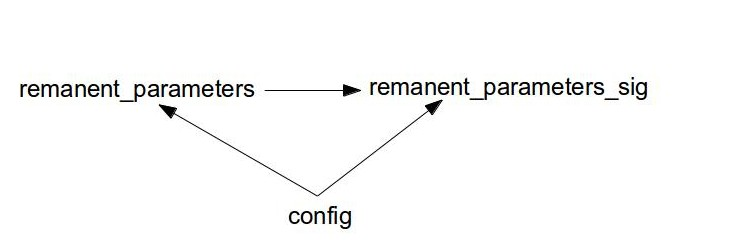
\includegraphics[width=80mm]{config.jpg}
\end{figure}

\item \verb|data_structures|

\begin{i}
\item \verb|int_inf|: unbounded integer library, with infinity.
\item \verb|int_storage|: this library provides primitives to deal with
  storage functions.
\item \verb|set_and_map|: this library provides primitives to deal with
  \verb|Set| and \verb|Maps| of ordered elements; in the fashion of OCaml's
  Map: it provides efficient iterators.
\item \verb|dictionary|: this library provides primitives to deal with
  indexed set of values. During the construction membership; transaction,
  and new key can be handled in \verb|O(log n)|. After the construction key can
  be translated in \verb|O(1)|.
\item \verb|hash|: this library provides signature for hash tables and
  several implementations.
\end{i}

\item \verb|frontend/preprocess|
\begin{i}
\item \verb|handler|: primitives to use a kappa handler.
\item \verb|print_handler|: pretty print of ckappa handler. Print the
  information in ``Signature'': agents, sites, states, and duals. And print
  the contact map in the dot format.
\item \verb|ckappa_sig|: signature for prepreprocessing language ckappa.
\item \verb|cckappa_sig|: signature for prepreprocessing language ckappa.
\item \verb|print_cckappa|: pretty print of token library. Print the second
  part ``Compilation'': variables; rules: lhs, rhs, direct, reverse;
  actions: unbinding, 1/2 unbinding, deletion, creation, binding;
  observables; initial\_states; perturbations.
\item \verb|print_ckappa|: pretty print of \verb|ckappa_sig|.

\item \verb|prepreprocess|: translation from KaSim ast to ckappa
  representation.
\item \verb|preprocess|: translation from KaSim ast to OpenKappa internal
  representation, and linkage.
\item \verb|list_tokens|: number agents, sites, states in ckappa
  representations.
\end{i}

\end{e}
















\end{document}